\documentclass[11pt,twoside,a4paper]{article}
\usepackage[margin=1in]{geometry}
\usepackage{verbatim}
\usepackage[justification=centering]{subfig}
\usepackage{graphicx}
\usepackage{url} % typeset URL's reasonably
\usepackage{listings}

\usepackage{pslatex} % Use Postscript fonts
\usepackage{algorithm}
\usepackage{algpseudocode}
%\usepackage[]{algorithm2e}
%\usepackage{subcaption}
\usepackage{color}
\usepackage{multirow}
\usepackage{makecell}

\usepackage{mathptmx}
\usepackage{amsmath}

\usepackage{appendix}
%define some own functions
\newcommand{\tabincell}[2]{\begin{tabular}{@{}#1@{}}#2\end{tabular}} 
\def\D{\mathrm{d}}


\begin{document}

	\title{Training Spiking Restricted~Boltzmann~Machine by Minimising Contrastive~Divergence}
	\author{
	Qian~Liu
	\thanks{
	The author is with the School of Computer Science, University of Manchester, Manchester M13 9PL, U.K. 
	(e-mail:qian.liu-3@manchester.ac.uk}
	}
	\maketitle
	\thispagestyle{empty}

\begin{abstract}
	In order to implement training of Spiking Deep~Belief~Networks~(SDBNs) on SpiNNaker, this paper studies the layer-by-layer training of spiking Restricted~Boltzmann~Machine~(RBM) of a DBN.
	The study starts from understanding the original problem, Products of Experts~(PoE), which was solved by using Contrastive~Divergence~(CD).
	It involves utilising Markov~Chain~Monte~Carlo~(MCMC) sampling to present the distribution of a certain untraceable high-dimensional probability model function, e.g. PoE.
	Among these sampling algorithms, Gibbs method is introduced and used in PoE problem.
	Instead of minimising the original objective function of Kullback-Leibler divergence, the contrastive divergence is exploited to solve PoE.
	Then the study continues on applying CD to RBM.
	Finally, on-line learning methods only spiking neurons used are explored to train spiking RBM.
\end{abstract}

\section{Why CD(Contrastive Divergence)?\cite{hinton2002training,woodfordnotes}}
	The probability of a vector point $ \mathbf{x} $ is modelled by the function $f(\mathbf{x} \mid \Theta )$ given the model parameters $ \Theta $, and normalised by a partition function $Z( \Theta)$:
	
	\begin{equation}
	p(\mathbf{x} \mid \Theta ) = \dfrac{f(\mathbf{x} \mid \Theta )}{Z( \Theta)}
	\end{equation}
	where the partition function is defined as:
	\begin{equation}
	\label{equ:z_int}
	Z( \Theta) = \int f(\mathbf{x} \mid \Theta )\D\mathbf{x}, \text{when  $ \mathbf{x} $ is continuous, or}
	\end{equation}
	
	\begin{equation}
	\label{equ:z_dis}
	Z( \Theta) = \sum_{\mathbf{x}} f(\mathbf{x} \mid \Theta ), \text{when  $ \mathbf{x} $ is discrete.}
	\end{equation}
	Given a set of data points $ \mathbf{D}=(\mathbf{d}_1, \mathbf{d}_2, ..., \mathbf{d}_K) $ the purpose of learning is to tune the model parameter $ \Theta $ to fit the data $ \mathbf{D}  $. 
	The objective function is the probability product of all the independent data points of the data set, which is also called the likelihood function:
	\begin{equation}
	 L (\Theta \mid \mathbf{D}) = p(\mathbf{D} \mid \Theta ) = \prod_{k=1}^K p(\mathbf{d}_k \mid \Theta ) =  \prod_{k=1}^K\dfrac{f(\mathbf{d}_k \mid \Theta )}{Z( \Theta)}.
	\end{equation}
	 And the target is to maximise the likelihood given the data set $ \mathbf{D}  $, which equals to maximise the log of the probability product (the log-likelihood):
	\begin{equation}
	    \log  L (\Theta \mid \mathbf{D}) = \log p(\mathbf{D} \mid \Theta ) = \sum_{k=1}^K\log f(\mathbf{d}_k \mid \Theta ) - K \log Z( \Theta),
	\end{equation}
	or the average log-likelihood:
	\begin{equation}
	\label{equ:like}
		\hat{l} (\Theta \mid \mathbf{D}) =\frac{1}{K}\log  L (\Theta \mid \mathbf{D}) 
		=\frac{1}{K}\sum_{k=1}^K\log f(\mathbf{d}_k \mid \Theta ) - \log Z( \Theta).
	\end{equation}
	Imagine three different conditions (probability function) as following.
	
	\textbf{First}, $f(\mathbf{x} \mid \Theta )$ is the probability density function (pdf) of a normal distribution $\mathcal{N}(x \mid \mu, \sigma )$.
	Data vector $ \mathbf{x} $ is just a one dimensional data point, $x$.
	$ Z( \Theta) $ equals to 1, thus $p(x \mid \Theta ) = \mathcal{N}(x \mid \mu, \sigma )$.
	\begin{equation}
	\hat{l} (\Theta \mid D) =  
	\frac{1}{K} \sum_{k=1}^K \log \left[ \frac{1}{\sigma \sqrt{2\pi}} \exp(-\frac{(d_k-\mu)^{2}}{2\sigma^{2}}) \right]
	\label{pdf}
	\end{equation}
	To maximise Equation~\ref{pdf} is to find the Maximum Likelihood Estimation (MLE) of parameters $ \mu $ and $ \sigma $, by deriving from the partial differential equations when they are equal to 0. 
	\begin{equation}
	\left\{
	\begin{aligned}
	   &\dfrac{\partial \hat{l} (\Theta \mid D)}{\partial \mu}= \sum_{k=1}^K -\frac{1}{2\sigma^{2}}\dfrac{\partial (\mu-d_k)^{2}}{\partial \mu} = \sum_{k=1}^K -\frac{1}{\sigma^{2}}(\mu-d_k) = 0 \quad\\
	   &\dfrac{\partial \hat{l} (\Theta \mid D) }{\partial \sigma^{2}}= -\frac{K}{2\sigma^{2}}+\frac{1}{2\sigma^{4}}\sum_{k=1}^K d_k^{2} -\frac{\mu}{\sigma^{4}}\sum_{k=1}^K d_k + \frac{K\mu^{2}}{2\sigma^{4}} = 0 \quad\\
	\end{aligned}
	\right.
	\end{equation}
	\begin{equation}
	\left\{
	\begin{aligned}
	    &\mu= \frac{1}{K}\sum_{k=1}^K d_k  \quad\\
	    &\sigma^{2} = \frac{1}{K}\sum_{k=1}^K d_k^{2} - (\frac{1}{K}\sum_{k=1}^K d_k)^{2}
	\end{aligned}
	\right.
	\end{equation}
	$\hat{l} (\Theta \mid D)$ here is the function of two dimensional parameters $\mu$ and $\theta$, and searching the highest point in the parameter space ``is equivalent to being in the field on a clear, sunny day,''~\cite{woodfordnotes} seeing the point straight away.
	
	\textbf{Second}, the probability model function changes to be the sum of N normal distributions: 
	\begin{equation}
	f(x \mid \Theta ) = \sum_{i=1}^N\mathcal{N}(x \mid \mu_i, \sigma_i ).
	\end{equation}
	Derived from Equation~(\ref{equ:like}), the objective function is:
	\begin{equation}
	\hat{l} (\Theta \mid D) = \frac{1}{K}\sum_{k=1}^K \log \sum_{i=1}^N \mathcal{N}(d_k \mid \mu_i, \sigma_i ) - \log N,
	\end{equation}
	where $\log Z( \Theta)$ still equals a constant, but the partial differential equation of any parameter depends on other model parameters.
	It is very hard to solve equation set of log of sum, thus iteration methods are introduced, e.g., gradient descent method. %and expectation maximization (EM) algorithm
	Searching for a local maximum of the likelihood function in the parameter space starts with an initial point, either random or well selected.
	For each iteration, the partial derivatives for every dimension of the parameter point are calculated as the gradient.
	The gradient determines the decent direction of the space search, the next parameter point is one step $ \eta $  towards the direction or is the highest point found by line search.
	
	The gradient descent method is equivalent to ``being in the field at night with a torch.''~\cite{woodfordnotes}.
	And then the descent direction is estimated and chosen by using the torch to see the relative heights of the field a short distance in each direction.
	Because partial differential equation of any parameter depends on other model parameters, we can only see the gradient for a small area.
	The search will follow the direction by walking one step or a certain distance (e.g. line search lowest point), and then start a new iteration.
	

\subsection{PoE Problem}
	\textbf{Finally}, the probability model function becomes the product of N normal distributions: 
	\begin{equation}
	f(x \mid \Theta ) = \prod_{i=1}^N\mathcal{N}(x \mid \mu_i, \sigma_i ),
	\end{equation}
	where the partition (normalisation) function $Z( \Theta)$ is no longer a constant, but varies accordance to all the parameters.
	Essentially, the integration of the probability model, see Equation~(\ref{equ:z_int}) and~(\ref{equ:z_dis}), is usually algebraically intractable.
	We have to use numerical integration method to evaluate the Equation~(\ref{equ:like}), whose partial derivative is (we are using vectors to generalise the problem):
	\begin{equation}
	\label{equ:part}
	\begin{aligned}
	\dfrac{\partial \hat{l} (\Theta \mid \mathbf{D})}{\partial \theta} 
	& = \frac{1}{K} \dfrac{\partial \sum_{k=1}^K\log f(\mathbf{d}_k \mid \Theta )}{\partial \theta} - \dfrac{\partial \log Z( \Theta)}{\partial \theta}\\
	& =  \frac{1}{K}\sum_{k=1}^K \dfrac{\partial \log f(\mathbf{d}_k \mid \Theta)}{\partial \theta} - \int p(\mathbf{x} \mid \Theta) \dfrac{\partial \log f(\mathbf{x} \mid \Theta)}{\partial \theta} \D \mathbf{x}\\
	& = \left \langle \dfrac{\partial \log f(\mathbf{d} \mid \Theta)}{\partial \theta}\right \rangle_{\mathbf{D}} -\left \langle \dfrac{\partial \log f(\mathbf{c} \mid \Theta)}{\partial \theta}\right \rangle_{\mathbf{C} \sim p(\mathbf{x} \mid \Theta)}  \\
	&=\left \langle \dfrac{\partial \log f(\mathbf{x} \mid \Theta)}{\partial \theta}\right \rangle_{\mathbf{X}_{data}} - \left \langle \dfrac{\partial \log f(\mathbf{x} \mid \Theta)}{\partial \theta}\right \rangle_{\mathbf{X}_{model}},
	\end{aligned}
	\end{equation}
	where  $ <\cdot>_x $ denotes the mean expectation of $ \cdot $ given distribution of $x$.
	The first term of the right-hand side is easy to get with the given data set $ \mathbf{D} $, and the second term can be approximated by generating data samples $ \mathbf{C} $ according to $ p(\mathbf{x} \mid \Theta) $.
	These generative samples is called ``fantasy data'' and can be generated using Monte Carlo Markov Chain (MCMC) sampling, see section~\ref{sec:mcmc}.
	The detailed derivation process can be found in Appendix~\ref{app:part}.
	Although in this example the integration of product of normal distribution is still tractable, it is also helpful to use numerical integration.

	Go back to the metaphor of the parameter field, solving PoE problem is like searching the highest point in a completely dark night without a torch.
	The computation of Equation~(\ref{equ:part}) is to ``feel the gradient of the field under our feet''.~\cite{woodfordnotes}.
	%The motivation underlining Contrastive Divergence algorithm is to boost the training speed of a Markov Chain in order to represent the distribution of a PoE (Product of Expert) model.
	%Thus the sampling can be followed using this trained Markov Chain model. 
\subsection{MCMC Sampling}
	\label{sec:mcmc}
	In order to solve the integration of algebraically intractable equations we can use numerical integration to approximate.
	One of the popular method is Monte Carlo integration:
	\begin{equation}
	\int_{a}^{b} f(x) \D x = \int_{a}^{b}\frac{f(x)}{q(x)}q(x)\D x = \dfrac{1}{N}\sum_{i=1}^{N}\frac{f(x_i)}{q(x_i)}.
	\end{equation}
	The integration of $ f(x) $ transforms to the integration of a new function $ F(x) = f(x)/q(x)  $ times its probability function $ q(x) $.
	It could be approximated by sampling N data points $ x_i $ according to the probability distribution $ q(x) $, and calculate the average of $ F(x_i) $ as $ <F(x)>_{q(x)}$.
	So the main question following is how to sample from a probability distribution.
	
	MCMC algorithm was proposed by Metropolis in 1953 and it became a wide-used sampling method.
	The stationary distribution $ \pi $ exists when every two nodes in a Markov Chain are connected regardless of the initial state distribution $ \pi_0 $:
	\begin{equation}
	\begin{aligned}
		&\pi(j) = \sum_{i=1}^{\infty}\pi(i)P_{ij} \\
		&\pi P = \pi,
	\end{aligned}
	\end{equation}
	where $ P $ is the transition probability matrix, and $ \pi $ is in the state space of a MC and the sum, $ \sum_{i=1}^{\infty}\pi(i) $,of a state distribution is 1.
	Thus based on the useful theorem of MC, sampled sequence $ \{x_0, x_1, ..., x_n, ... \}$ from a MC complies with its stationary distribution $ \pi(x) $.
	Metropolis stated that if a MC has a stationary distribution, $ q(x) $, which is exactly needed to sample from, then we can easily obtain a sample sequence along the MC according to the transformation probability matrix $ P $.
	Here so far we are describing the MC with discrete states, however the it also applies to continuous $ \pi $ and $ P $.
	The problem here is to build $ P $ to make the stationary distribution equal to the required probability, $ \pi(x) = q(x) $.
	
	So the other useful theorem (detailed balance) lies here, if an aperiodic MC is reversible: $\pi (i) P_{ij} = \pi (j) P_{ji},$ then $ \pi $ is the stationary distribution.
	It is a stronger condition than the previous theorem, so most of the MCs are not generally eligible:
	\begin{equation}
	\pi (i) P_{ij} \neq \pi (j) P_{ji}.
	\end{equation}
	Thus we can introduce another parameter matrix, $ \alpha $ to make a general MC reversible:
	\begin{equation}
	\pi (i) P_{ij} \alpha_{ij} = \pi (j) P_{ji} \alpha_{ji}	,
	\end{equation}
	where $ \alpha_{ij} = \pi(j) P_{ji} $ and $ \alpha_{ji} = \pi(i) P_{ij}$.
	The altered transformation probability matrix is $ P'_{ij} =  P_{ij} \alpha_{ij}$ and $ P'_{ji} =  P_{ji} \alpha_{ji}$, and the MC complies the detailed balance condition: $\pi (i) P'_{ij} = \pi (j) P'_{ji}$.
	The matrix parameter $ \alpha $ is called as ``acceptance rate'', and its physic meaning is as follows: when state $ i $ transforms to state $ j $ with a probability of $ P_{ij} $, the transformation is accepted by the rate of $ \alpha_{ij} $.
	Since the accept rate may be too low for the sampling to move along the MC, we can normalise the $ \alpha $ pair to 1:
	\begin{equation}
		\alpha^{'}(i,j) = min \left\{\frac{\pi(j)P_{ji}}{\pi(i)P_{ij}},1\right\}.
	\end{equation}
	The algorithm is called Metropolis-Hastings and described in following:
	\begin{algorithm}[h]
	  \caption{Metropolis-Hastings Sampling}
	  \label{alg:mcmc}
	  \begin{algorithmic}
	  	
%	    \Procedure{Correction}{coeffs $C$, correlations $Q$}
	    \State Initialisation $x_0 = s_{random}$, \Comment{$ x $:sampling sequence and $s$:state in MC}
	    \For{$t=1, 2, ..., N$}
		    \State $y \sim p_(x \mid x_{t-1})$ 
			    \Comment{Random drawing the next state by the transformation probability matrix $P$}
		    \State $ u \sim Uniform[0,1] $ 
			    \Comment{Random drawing from a uniform distribution}
			\If {$ u < \alpha^{'}(x_{t-1},y) = min \left\{\frac{q(y)p_(x_{t-1} \mid y)}{q(x_{t-1})p_(y \mid x_{t-1})},1\right\} $}
				\State {$x_t = y$} \Comment{Accept the transformation when the random number is less than $\alpha$}
				\Else \State {$x_t = x_{t-1}$}  \Comment{Transformation is refused elsewise}
			\EndIf
		\EndFor
	  \end{algorithmic}
	\end{algorithm}
	
	The probability model function as the product of N normal distributions can be approximated by using this Metropolis-Hastings sampling.
\subsection{Gibbs Sampling}
	\label{sec:Gibbs}
	For high dimensional data sampling, it is possible to make the accept rate to 1 which increases the convergence speed dramatically.
	According to conditional probability:
	\begin{equation}
		P(A \mid B) = \frac{P(A \cap B)}{P(B)}.
	\end{equation}
	For a $ n $ dimensional data $ (\mathbf{x}, y) $ where $ \mathbf{x}=(x_1,x_2,...,x_{n-1}) $, the joint probability of $p(\mathbf{x},y)$ is:
	\begin{equation}
		p(\mathbf{x},y) = p(y \mid \mathbf{x})p(\mathbf{x}).
	\end{equation}
	Thus, during sampling if we restrict the direction of transformation to one single axis(dimension), $ y $, from point $ A(\mathbf{x}_1, y_1) $ to point $ B(\mathbf{x}_1, y_2)$:
	\begin{equation}
		p(\mathbf{x}_1, y_1)p(y_2 \mid \mathbf{x}_1) = p(\mathbf{x}_1, y_2)p(y_1 \mid \mathbf{x}_1) = p(\mathbf{x}_1)p(y_1 \mid \mathbf{x}_1)p(y_2 \mid \mathbf{x}_1),
	\end{equation}
	then, the MC obeys the condition of detailed balance.
	So the stationary distribution $ \pi(x_1,x_2,...,x_n) $ equals to the joint probability $ p(x_1,x_2,...,x_n) $ and the transformation probability matrix P is consisted of the conditional probability of each dimension $ k $ $,  p(x_k \mid x_1,...,x_{k-1},x_{k+1},...,x_n) $.
	Therefore, given the conditional distribution of each variable for a multivariate distribution Gibbs sampling is able to approximate the joint distribution with long enough sample sequence.
	Gibbs sampling is described as follows:
	\begin{algorithm}[h]
	  \caption{Gibbs Sampling}
	  \label{alg:gibbs}
	  \begin{algorithmic}
	  	
%	    \Procedure{Correction}{coeffs $C$, correlations $Q$}
	    \State Initialisation $\mathbf{x}_0 = [x_0(1),x_0(2),...,x_0(M)]$,  \Comment{Random initialise $\mathbf{x}_0$}
	    \For{$t=1, 2, ..., N$}
	    	\For{$k=1, 2, ..., M$}
	    		\State $ x_t(k) = p(x(k) \mid x_{t-1}(1),x_{t-1}(2),...,x_{t-1}(k-1),x_{t-1}(k+1),...,x_{t-1}(M))$\\
	    		\Comment{Sampling by the conditional distribution}
			\EndFor
		\EndFor
	  \end{algorithmic}
	\end{algorithm}
	
\subsection{CD Instead of KL(Kullback-Leibler)}
\label{sec:CD}
	Kullback-Leibler divergence is the measure of how different two probability distributions are:
	\begin{equation}
	\begin{aligned}
	KL(P \mid \mid Q)
	&= \int P(\mathbf{x}) \log \frac{P(\mathbf{x})}{Q(\mathbf{x})} \D \mathbf{x}\\
	%= \sum_{\mathbf{x}} P(\mathbf{x}) \log \frac{P(\mathbf{x})}{Q(\mathbf{x})} \\
	&= \int P(\mathbf{x}) \log P(\mathbf{x}) \D \mathbf{x} - \int P(\mathbf{x}) \log Q(\mathbf{x}) \D \mathbf{x}\\
	%=  \sum_{\mathbf{x}} P(\mathbf{x}) \log P(\mathbf{x}) - \sum_{\mathbf{x}} P(\mathbf{x}) \log Q(\mathbf{x})\\
	&= \left \langle \log P(\mathbf{x}) \right \rangle_{\mathbf{X} \sim P(\mathbf{x})} - \left \langle \log Q(\mathbf{x}) \right \rangle_{\mathbf{X} \sim P(\mathbf{x})} ,
	\end{aligned}
	\end{equation}
	and the second term of the right hand side is the average log-likelihood function (see Equation~\ref{equ:like}) if $P(\mathbf{x})$ is the training data distribution and $Q(\mathbf{x})$ is the model distribution:
	\begin{equation}
	\begin{aligned}
	& KL \left( p(\mathbf{x} \mid \mathbf{D}) \mid \mid p(\mathbf{x} \mid \Theta) \right)
	=   \left \langle \log p(\mathbf{d} \mid \mathbf{D}) \right \rangle_{\mathbf{D}} - \left \langle \log p(\mathbf{d} \mid \Theta) \right \rangle_{\mathbf{D}}, \textit{where} \\
	& \hat{l} (\Theta \mid \mathbf{D}) =\frac{1}{K}\log  L (\Theta \mid \mathbf{D}) 
	=  \frac{1}{K}\log p(\mathbf{D} \mid \Theta ) 
	= \frac{1}{K} \sum_{k=1}^{\mathbf{K}} \log f(\mathbf{d}_k \mid \Theta )
	= \left \langle \log p(\mathbf{d} \mid \Theta) \right \rangle_{\mathbf{D}}.
	\end{aligned}
	\end{equation}
	We use $ \mathbf{D} $ instead of $ \mathbf{X} \sim p(\mathbf{x} \mid \mathbf{D}) $, for $ p(\mathbf{x} \mid \mathbf{D}) $ is the distribution of data set $ \mathbf{D} $.
	If we need to generate a sample sequence according to the distribution $ p(\mathbf{x} \mid \mathbf{D}) $, $ \mathbf{D} $ itself is the most approximated.
	Since $\left \langle \log p(\mathbf{d} \mid \mathbf{D}) \right \rangle_{\mathbf{D}}$ is independent with model parameters, the negative partial derivative is the same with Equation~(\ref{equ:part}):
	\begin{equation}
	\label{equ:kl}
		-\dfrac{\partial KL \left( p(\mathbf{x} \mid \mathbf{D}) \mid \mid p(\mathbf{x} \mid \Theta) \right)}{\partial \theta}
		= \dfrac{\partial \hat{l} (\Theta \mid \mathbf{D})}{\partial \theta} \\
		= \left \langle \dfrac{\partial \log f(\mathbf{d} \mid \Theta)}{\partial \theta}\right \rangle_{\mathbf{D}} - \left \langle \dfrac{\partial \log f(\mathbf{c} \mid \Theta)}{\partial \theta}\right \rangle_{\mathbf{C} \sim p(\mathbf{x} \mid \Theta)} .
	\end{equation}
	Therefore, for each iteration searching in the parameter space we use $ k $ number of training data $ \mathbf{D}=(\mathbf{d}_1, \mathbf{d}_2, ..., \mathbf{d}_k) $ and fantasy data $ \mathbf{C}=(\mathbf{c}_1, \mathbf{c}_2, ..., \mathbf{c}_k) $.
	If $ k $ is big enough, sampling sequences $ \mathbf{D} $ and $ \mathbf{C} $ are able to approximate the data and the model distribution thus to get derivatives of the KL function.
	However, if we just take a small number of data, even $ k = 1 $ per iteration~\cite{hinton2002training}, the KL divergence can be seen as a ``k-step contrastive convergence ($ CD_{k}) $'':
	\begin{equation}
	\label{equ:cdk}
		\dfrac{\partial CD_{k}}{\partial \theta} 
		= - \left \langle \dfrac{\partial \log f(\mathbf{d} \mid \Theta)}{\partial \theta}\right \rangle_{(\mathbf{d}_1, \mathbf{d}_2, ..., \mathbf{d}_k) } + \left \langle \dfrac{\partial \log f(\mathbf{c} \mid \Theta)}{\partial \theta}\right \rangle_{(\mathbf{c}_1, \mathbf{c}_2, ..., \mathbf{c}_k) \sim p(\mathbf{x} \mid \Theta)}.
	\end{equation}
	Since the searching step $ \eta $ is very small, the derivatives of points in a small area can be seen as the same.
	The step made for a single $ CD_{k} $ can be approximated by summation of $ k $ steps of $ CD_{1} $ as long as the searching does not go far.
	Otherwise the searching path may follow some direction for accumulated steps away from the original area, thus significantly reduces the training time.
	
	Although there is reasonable explanation on using $CD_1$ for parameter space searching, arguments exist over whether the search converge to the same maxima/minima as $CD_\infty$.
	As an initial exploration over the problem we tested some experiments on Section~\ref{sec:cd1}. 
%	Thus,
%	\begin{equation}
%		\dfrac{\partial [KL(p^0 \mid \mid p^{\infty}) - KL(p^1 \mid \mid p^{\infty})]}{\partial \theta}
%		= \left \langle \dfrac{\partial \log f(\mathbf{x} \mid \Theta)}{\partial \theta}\right \rangle_{\mathbf{p}^1} - \left \langle \dfrac{\partial \log f(\mathbf{x} \mid \Theta)}{\partial \theta}\right \rangle_{\mathbf{p}^0},
%	\end{equation}
%	where the second term in equation~(\ref{equ:kl}) cancels out.
%	So Hinton proposed \textcolor{red}{the new contrastive divergence CD to make Gibbs sampling with only 1 step}.
%	Contrastive divergence is defined as:
%	\begin{equation}
%		CD_n = KL(p^0 \mid \mid p^{\infty}) - KL(p^n \mid \mid p^{\infty})
%	\end{equation}
\section{RBM\cite{zhang2013rbm}}
	RBM is a restricted version of Boltzman machine, where there are only connections between layers of units but not between units within a layer, see Figure~\ref{fig:RBM}.
	$ v $ is the layer of visible units representing the observable data $ \mathbf{v} $, while $ h $ are the hidden units which can be seen as feature extractors.
	The connections between the hidden layer and the visible layers are bidirectional weights, $ \mathbf{W} $.
	Note that, both visible and hidden units have their bias individually, $ \mathbf{a} $ and $ \mathbf{b} $.
	Thus the RBM consists of the data $ \mathbf{D} = \mathbf{V} = (\mathbf{v}_1, \mathbf{v}_2, ..., \mathbf{v}_K ) $, the model parameters $ \Theta = (\mathbf{a}, \mathbf{b}, \mathbf{W}) $ and the hidden units $ \mathbf{h} \sim p(\mathbf{h} \mid \mathbf{v}, \Theta) $.
	\begin{figure}[hbt]
	\centering
		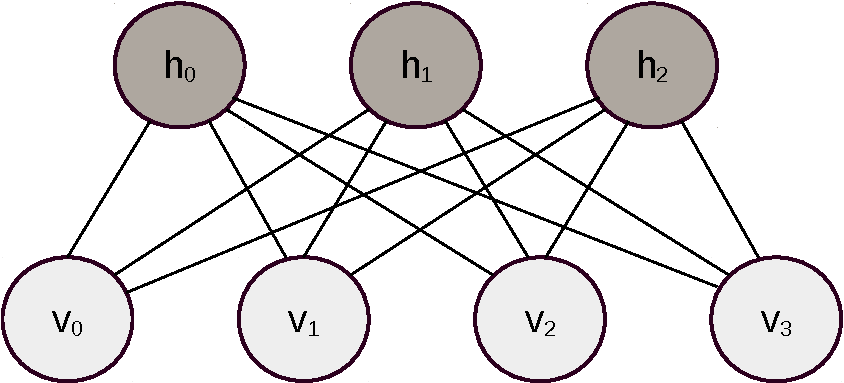
\includegraphics[width=0.6\textwidth]{img/RBM.pdf}
		\caption{A typical RBM structure.}
		\label{fig:RBM}
	\end{figure}
	
	The Energy function~\cite{hopfield1982neural} of a RBM is defined as follows, which has $ n $ vision units and $ m $ hidden ones:
	\begin{equation}
		E(\mathbf{v}, \mathbf{h} \mid \Theta)= -\sum_{i=1}^n a_i v_i - \sum_{j=1}^m b_j h_j - \sum_{i=1}^n \sum_{j=m}^n v_i W_{ij} h_j.
	\end{equation}
	And the model function and its probability functions are as follows:
	\begin{equation}
		\begin{aligned}
		& f(\mathbf{v}, \mathbf{h} \mid \Theta) =e^{-E(\mathbf{v}, \mathbf{h} \mid \Theta)} \\
		& p(\mathbf{v}, \mathbf{h} \mid \Theta) =\frac{e^{-E(\mathbf{v}, \mathbf{h} \mid \Theta)}}{Z(\Theta)}\\
		& Z(\Theta) = \sum_{\mathbf{v}} \sum_{\mathbf{h}} e^{-E(\mathbf{v}, \mathbf{h} \mid \Theta)}.
		\end{aligned}
	\end{equation}
	Note that, the model function $ f(\mathbf{v}, \mathbf{h} \mid \Theta) $ is nicely defined as a PoE problem, and each hidden unit represent an expert.
	However, we are more interested in the marginal probability function: $ p(\mathbf{v} \mid \Theta) $:
	\begin{equation}
		p(\mathbf{v} \mid \Theta) =\frac{\sum_{ \mathbf{h}} e^{-E(\mathbf{v}, \mathbf{h} \mid \Theta)}}{Z(\Theta)}.
	\end{equation}		
\subsection{Objective Function}
	Although $ p(\mathbf{v} \mid \Theta) $ is not a PoE problem, the partial derivation of the average log-likelihood function still applies to Equation~(\ref{equ:part}) and the intractable integration is the same problem here:
	\begin{equation}
		\label{equ:RBM}
		\begin{aligned}
		\dfrac{\partial \hat{l} (\Theta \mid \mathbf{D})}{\partial \theta} 
		& = \left \langle \dfrac{\partial -E(\mathbf{v}, \mathbf{h} \mid \Theta)}{\partial \theta} \right \rangle_{\mathbf{h} \sim p( \mathbf{h} \mid \mathbf{v}, \Theta), \mathbf{V}} 
		- \left \langle \dfrac{\partial -E(\mathbf{v}, \mathbf{h} \mid \Theta)}{\partial \theta} \right \rangle_{\mathbf{v}, \mathbf{h} \sim p( \mathbf{v}, \mathbf{h} \mid  \Theta)},  \\
		\end{aligned}
	\end{equation}
	The detailed derivation process, please see Appendix~\ref{app:RBM}.
	Regarding the specific RBM parameters,  $ \Theta = (\mathbf{a}, \mathbf{b}, \mathbf{W}) $, the derivatives are:
	\begin{equation}
		\label{equ:RBM_2}
		\begin{aligned}
		\dfrac{\partial \hat{l} (\Theta \mid \mathbf{D})}{\partial W_{ij}} 
		& = \left \langle v_i h_j \right \rangle_{\mathbf{h} \sim p( \mathbf{h} \mid \mathbf{v}, \Theta), \mathbf{V}} 
		- \left \langle  v_i h_j \right \rangle_{\mathbf{v}, \mathbf{h} \sim p( \mathbf{v}, \mathbf{h} \mid  \Theta)},  \\
		\dfrac{\partial \hat{l} (\Theta \mid \mathbf{D})}{\partial a_{i}} 
		& = \left \langle v_i \right \rangle_{\mathbf{h} \sim p( \mathbf{h} \mid \mathbf{v}, \Theta), \mathbf{V}} 
		- \left \langle  v_i \right \rangle_{\mathbf{v}, \mathbf{h} \sim p( \mathbf{v}, \mathbf{h} \mid  \Theta)},  \\
		\dfrac{\partial \hat{l} (\Theta \mid \mathbf{D})}{\partial b_{j}} 
		& = \left \langle h_j \right \rangle_{\mathbf{h} \sim p( \mathbf{h} \mid \mathbf{v}, \Theta), \mathbf{V}} 
		- \left \langle  h_j \right \rangle_{\mathbf{v}, \mathbf{h} \sim p( \mathbf{v}, \mathbf{h} \mid  \Theta)},  \\
	\end{aligned}
	\end{equation}	 
	
\subsection{CD with 1-step Reconstruction}
	Both terms of the derivatives of the average log-likelihood function (Equation~(\ref{equ:RBM})) are intractable, so generative models for sampling is needed.
	As stated in Section~\ref{sec:CD}, for each iteration only one sample is generated.
	
	Regarding to the first term, given a training data $ \mathbf{v}_0 $ we first generate a hidden vector according to the conditional distribution $ \mathbf{h}_0 \sim p( \mathbf{h} \mid \mathbf{v}_0, \Theta) $.
	Welling et al. have proposed~\cite{welling2004exponential} that both the hidden and visible units can be any exponential unit, such as softmax, Gaussian and Poissonian.
	Here we take a Bernoulli-Bernoulli RBM as an example, where each node is a sigmoidal unit.
	The conditional probability function is as follows:
	\begin{equation}
		p(h_i = 1 \mid \mathbf{v}) = \sigma(\sum_{j=1}^{m} W_{ij} \cdot \mathbf{v} + b_j).
	\end{equation}
	
	The second term is perfect fit for Gibbs sampling, since we can $ p(\mathbf{v}, \mathbf{h} \mid \Theta) $ as a 2D vector and generating the samples by jumping in a Markov Chain with the transformation probability matrix $ p(\mathbf{v} \mid \mathbf{h}, \Theta) $ and $ p(\mathbf{h} \mid \mathbf{v}, \Theta) $, see Figure~\ref{fig:gibbs} and Section~\ref{sec:Gibbs}.
	So, with the given data $ \mathbf{v}_0 $ and the sampling data $ \mathbf{h}_0 $, we have the initial data point in this Markov Chain,  ($ \mathbf{v}_0, \mathbf{h}_0$).
	The transformation starts from the axis of $ \mathbf{v} $, then we get $ \mathbf{v}_1 \sim p( \mathbf{v} \mid \mathbf{h}_0, \Theta) $.
	It follows the next axis $ \mathbf{h} $, similarly we get $ \mathbf{h}_1 \sim p( \mathbf{h} \mid \mathbf{v}_1, \Theta) $.
	So far we obtain the first sample along the Markov Chain, ($ \mathbf{v}_1, \mathbf{h}_1$) thus to solve the objective function with one iteration.
	The algorithm is described below:   
	\begin{algorithm}[h]
		\caption{Learning on RBM Parameters with $ CD_1 $}
		\label{alg:learn}
		\begin{algorithmic}
%			\State Initialisation $\mathbf{x}_0 = [x_0(1),x_0(2),...,x_0(M)]$,  \Comment{Random initialise $\mathbf{x}_0$}
			\For{$t=1, 2, ..., K$} \Comment{K number of training data $ \mathbf{V} $, 1 data each iteartion}
%			\For{$k=1, 2, ..., M$}
			\State $ \mathbf{h}_t \sim p( \mathbf{h} \mid \mathbf{v}_t, \Theta) $
			\Comment{Generate $ \mathbf{h}_t $ given $ \mathbf{v}_t $ }
			\State $ \mathbf{v}_{t+1} \sim p( \mathbf{v} \mid \mathbf{h}_{t}, \Theta) $
			\Comment{Generate $ \mathbf{v}_{t+1} $ on v axis using Gibbs sampling }
			\State $ \mathbf{h}_{t+1} \sim p( \mathbf{h} \mid \mathbf{v}_{t+1}, \Theta) $
			\Comment{Generate $ \mathbf{h}_{t+1} $ on h axis using Gibbs sampling }
			\State $ \dfrac{\partial \hat{l} (\Theta \mid \mathbf{D})}{\partial W_{ij}} = v_{t,i} h_{t,j} - v_{t+1,i} h_{t+1,j}$
			\State $ \dfrac{\partial \hat{l} (\Theta \mid \mathbf{D})}{\partial a_{i}} = v_{t,i} - v_{t+1,i} $
			\State $  \dfrac{\partial \hat{l} (\Theta \mid \mathbf{D})}{\partial b_{j}} = h_{t,j} - h_{t+1,j}$
			\State $ \Delta W_{ij} = \eta ( v_{t,i} h_{t,j} - v_{t+1,i} h_{t+1,j}) $
			\Comment{Update $ W_{ij} $}
			\State $ \Delta a_{i} = \eta ( v_{t,i} - v_{t+1,i}) $
			\Comment{Update $ a_{i} $}
			\State $ \Delta b_{j} = \eta ( h_{t,j} - h_{t+1,j}) $
			\Comment{Update $ b_{j} $}
%			\EndFor
			\EndFor
		\end{algorithmic}
	\end{algorithm}
	\begin{figure}[hbt]
		\centering
		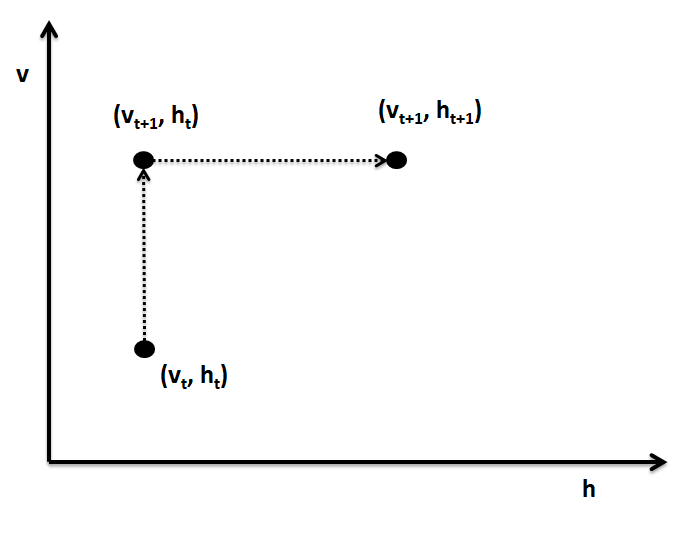
\includegraphics[width=0.5\textwidth]{img/gibbs.png}
		\caption{Gibbs sampling on RBM.}
		\label{fig:gibbs}
	\end{figure}	
\subsection{$CD_1$ vs $CD_{\infty}$}
\label{sec:cd1}
The common validation of trained RBMs is to measure the reconstruction error over the training dataset.
To be precise, the reconstruction of some training vision data $ v_0 $ is one step Gibbs sampling (from $ v_0 $ via $ (v_0, h_0 )$ to $ (v_1, h_0 )$) away from it, $ v_1 $.
We use the MNIST dataset as both the training and testing data.
The size of every image in MNIST is $28 \times 28$, and every pixel is with grey scale from 0 to 255.
To make it fit the binary status of the neurons, the pixels whose values over 50 are set as 1 and the others are set to 0, see Figure~\ref{Fig:5} as an example.
This RBM is with $28 \times 28$ visible units and 500 hidden units.
If we look at the measured results in Figure~\ref{Fig:error}, it is not surprise to see there is no obvious difference on the reconstruction error among $CD_1$, $CD_2$ and $CD_{1000}$.

	\begin{figure}[hbt]
		\centering
		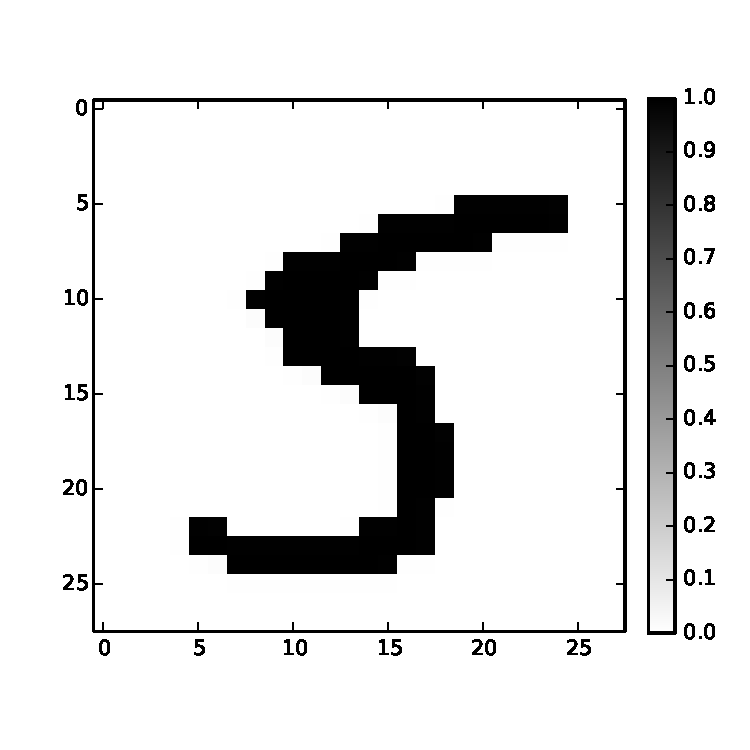
\includegraphics[width=0.5\textwidth]{img/test.pdf}
		\caption{An example of binary image in MNIST.}
		\label{Fig:5}
	\end{figure}

The objective function, Equation~(\ref{equ:cdk}), targets at maximise the log likelihood of data and model.
In another word, the samples generated from the converged model should have the same distribution as the training dataset.
However, lower reconstruction error means smaller changes over the first step of Gibbs sampling, where only one sample generated from the model.
It is impossible to compare two distributions with merely single data.

Thus, we have done another simple test to generate long sample sequence using Gibbs sampling.
In order to measure the distribution in a very naive way, we calculated the mean for every pixel in the training data and the generated sample sequence.
Then, the euclidean distance between the two matrix is given to roughly compare the distribution.

\begin{figure}[hbt]
  \centering
  \subfloat[Reconstruction error over training images, plotted only for the first $20,000$ searching steps.]{
    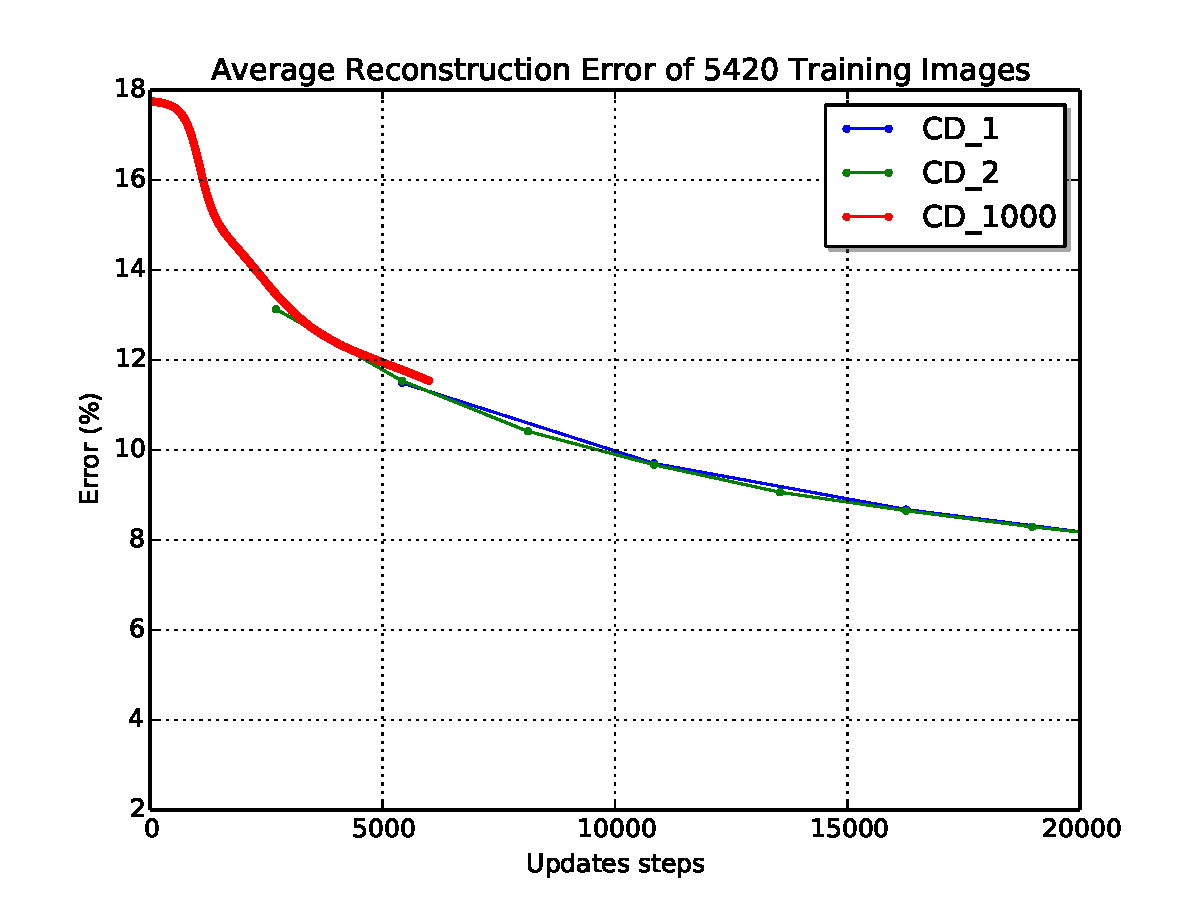
\includegraphics[width=0.4\textwidth]{img/train_short.pdf}
  }
  \subfloat[Reconstruction error over training images]{
      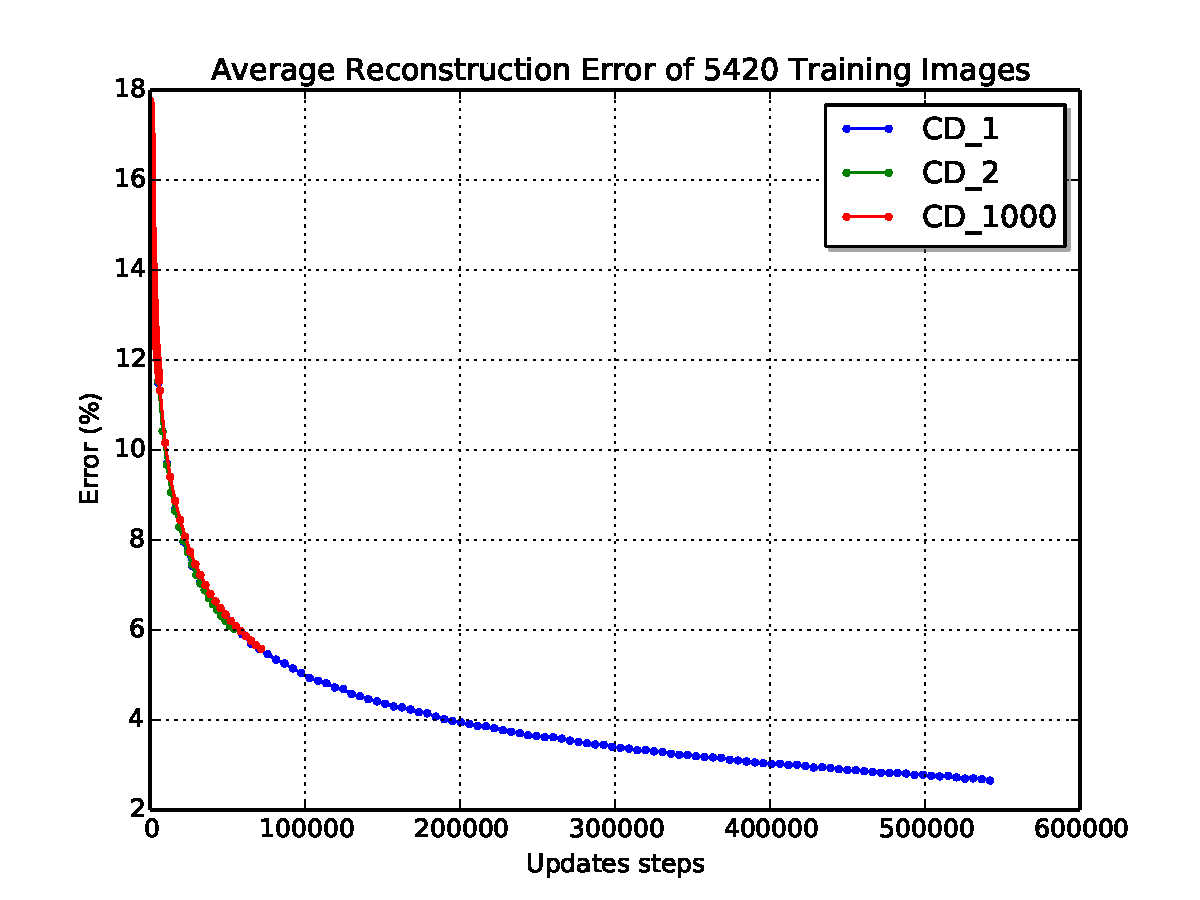
\includegraphics[width=0.4\textwidth]{img/train_long.pdf}
  }\\
 \subfloat[Reconstruction error over testing images, plotted only for the first $20,000$ searching steps.]{
     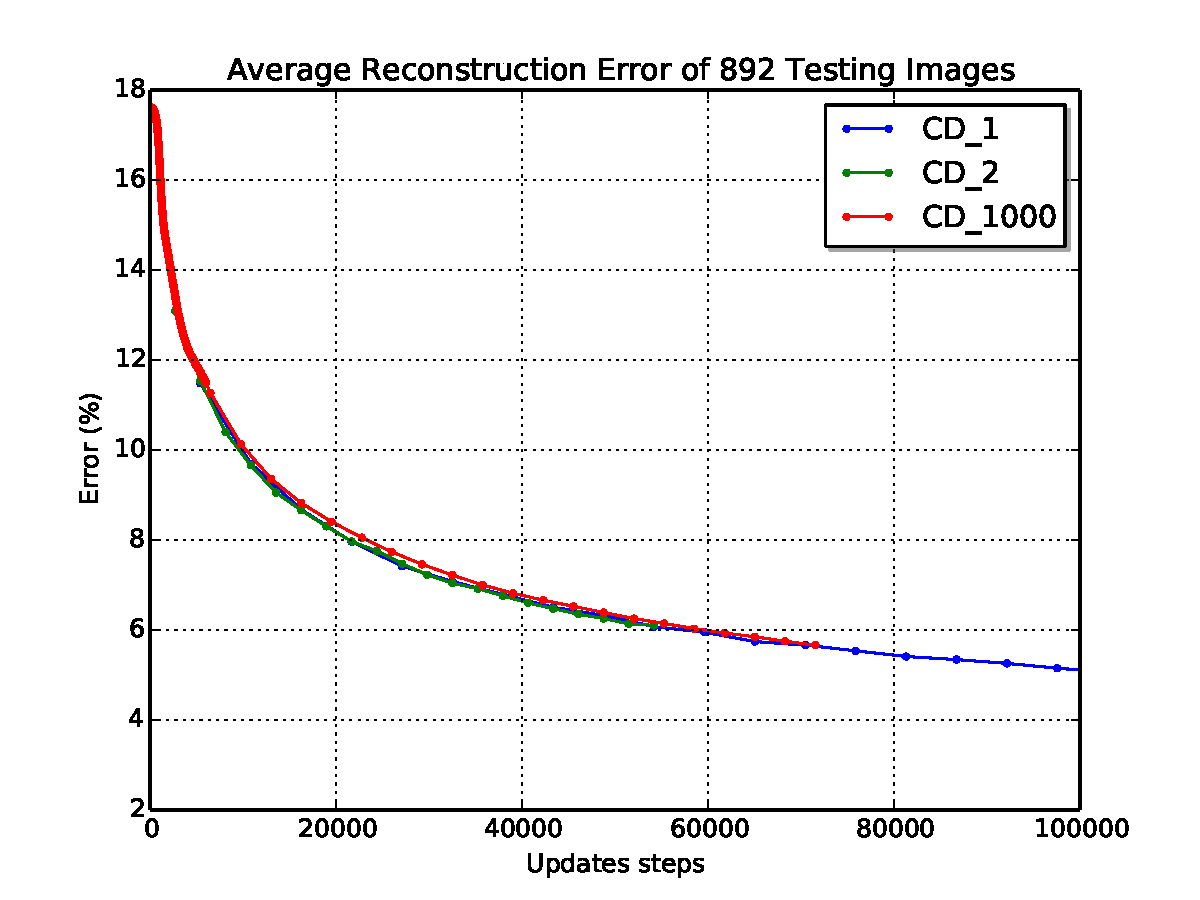
\includegraphics[width=0.4\textwidth]{img/test_short.pdf}
   }
   \subfloat[Reconstruction error over testing images]{
       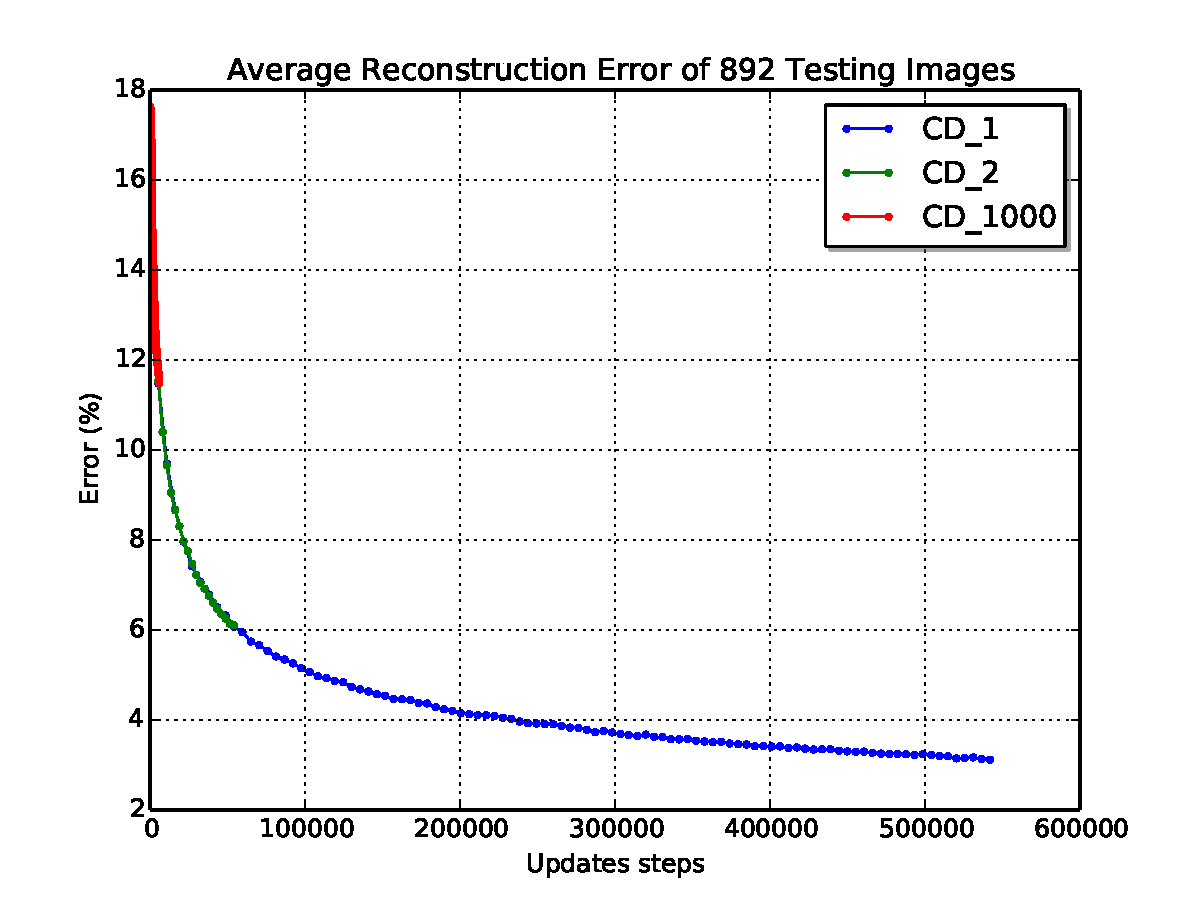
\includegraphics[width=0.4\textwidth]{img/test_long.pdf}
   }
  \caption{
  Reconstruction error.
  Due to the high cost of training with $CD_{1000}$, we stopped at $6,000$ update steps.
  }
  \label{Fig:error}
\end{figure}

In Figure~\ref{Fig:dis} we can see the obvious approximation with $CD_{1000}$.
There are 10 trails experimented for 5 configuration on sample size. 
	\begin{figure}[hbt]
		\centering
		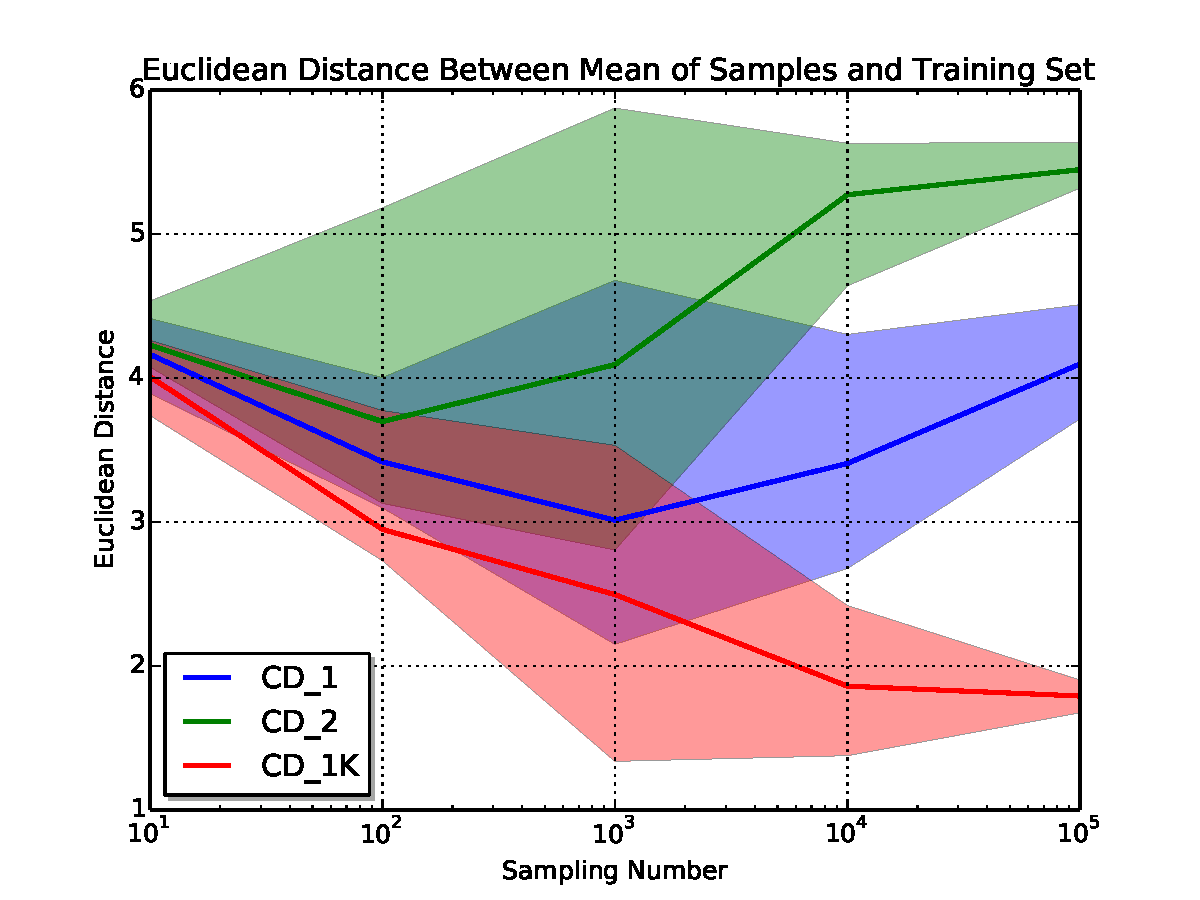
\includegraphics[width=0.7\textwidth]{img/distr.pdf}
		\caption{Euclidean distance between the training data and the generated Gibbs sampling sequence on the mean value only.} 
		\label{Fig:dis}
	\end{figure}
\section{Deep Belief Network}
The Deep Belief Network (DBN) model is proposed by Hinton et al.~\cite{hinton2006fast} in 2006, in which the top RBM (top two layers) works as an associative memory where the lower layers form a belief net with directed connections, see Figure~\ref{Fig:5}. \textcolor{red}{Need to redraw}
The main advantages of DBN comparing to multilayer perceptron (MLP) lie on the following:
	\begin{itemize}
	  \item \textbf{is a probabilistic model}, which not only presents $p(output \mid input)$ but also $p(input \mid output)$.
	  The deep layers work as complementary prior and solves the explain away problem in a belief net.
	  \textcolor{red}{Probably we need to start from explaining belief net and then the explain away problem as well as the complementary prior, and finally the probabilistic representations of DBN. }  
	  \item \textbf{works bidirectionally}, both down-top (recognition pass) and top-down (generative pass).
	  The generative model is able to reconstruct the input thus to interpret the hidden representations visibly.
	  \item \textbf{is trained with fast and unsupervised learning algorithm}.
	  As stated above RBM is trained in an unsupervised way with fast training algorithm targeting at CD.
	  Notice that although the lower layers are not RBMs, they can be pre-trained as RBMs.
%	  \textcolor{red}{??? During fine-tuning, every layer generates (reconstructs) its input with a probability of $p(input \mid output)$, the error between the input and the reconstruction makes the tuning on the generative pass exactly like back propagation (BP) but with only one layer.
%	  The same applies to the recognition pass}.
	  It also works with labelled data where the generative model presents both the labels and the data. 
	\end{itemize}
	\begin{figure}[hbt]
		\centering
		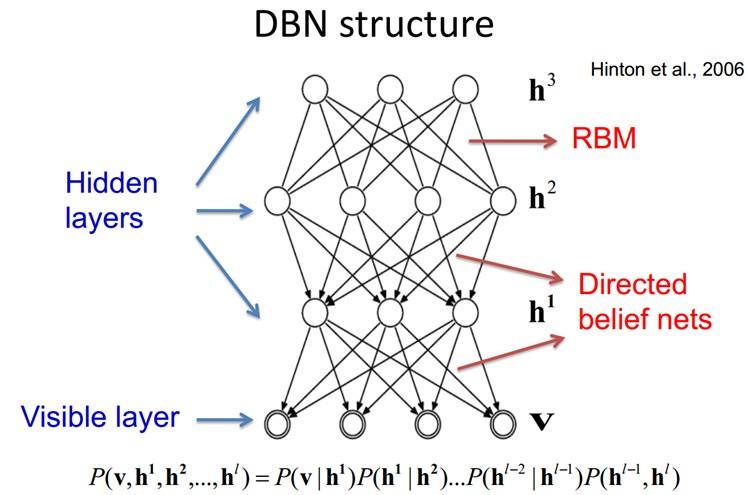
\includegraphics[width=0.7\textwidth]{img/dbn.jpg}
		\caption{A DBN contains undirected RBM on the top as an associative memory and directed belief net on the lower layers.} 
		\label{Fig:dbn}
	\end{figure}
	\subsection{A Probabilistic Representation}
	\subsection{Greedy Algorithm}
	\subsection{Case Study on Labelled Data}
	There is no unified training methods for DBN, here we reproduce the same example and training algorithm from the paper~\cite{hinton2006fast} in order to apply greedy training on lower layers, $CD_1$ on the top associative memory and fine-tuning bidirectionally.
	\subsection{Discussions on DBN Structure and Learning}
\section{Spiking RBM\cite{neftci2013event}}

\begin{appendices}
	\section{Derivation process of Equation~(\ref{equ:part})}
	\label{app:part}
		\begin{equation}
		\begin{aligned}
		 \dfrac{\partial \log Z(\Theta)}{\partial \theta}
		=&\frac{1}{Z(\Theta)}\dfrac{\partial Z(\Theta)}{\partial \theta}\\
		=&\frac{1}{Z(\Theta)} \int \dfrac{\partial f(\mathbf{x} \mid \Theta)}{\partial \theta} \D \mathbf{x} \\
		=&\frac{1}{Z(\Theta)} \int f(\mathbf{x} \mid \Theta) \frac{1}{f(\mathbf{x} \mid \Theta)} \dfrac{\partial  f(\mathbf{x} \mid \Theta)}{\partial \theta} \D \mathbf{x}\\
		=& \int \frac{f(\mathbf{x} \mid \Theta) }{Z(\Theta)} \dfrac{\partial \log f(\mathbf{x} \mid \Theta)}{\partial \theta} \D \mathbf{x}\\
		=& \int  p(\mathbf{x} \mid \Theta) \dfrac{\partial \log f(\mathbf{x} \mid \Theta)}{\partial \theta} \D \mathbf{x}\\
		=&\left \langle \dfrac{\partial \log f(\mathbf{c} \mid \Theta)}{\partial \theta}\right \rangle_{\mathbf{C} \sim p(\mathbf{x} \mid \Theta)}
		\end{aligned}
		\end{equation}
	\section{Derivation process of Equation~(\ref{equ:RBM})  }
	\label{app:RBM}
	\begin{equation}
		\begin{aligned}
		\dfrac{\partial \hat{l} (\Theta \mid \mathbf{D})}{\partial \theta} 
		& = \left \langle \dfrac{\partial \log f(\mathbf{d} \mid \Theta)}{\partial \theta}\right \rangle_{\mathbf{V=D}} -\left \langle \dfrac{\partial \log f(\mathbf{v} \mid \Theta)}{\partial \theta}\right \rangle_{\mathbf{V} \sim p(\mathbf{x} \mid \Theta)}  \\
		& = \left \langle \dfrac{\partial \log \sum_{ \mathbf{h}} e^{-E(\mathbf{v}, \mathbf{h} \mid \Theta)}}{\partial \theta}\right \rangle_{\mathbf{V}} 
		-\left \langle \dfrac{\partial \log \sum_{ \mathbf{h}} e^{-E(\mathbf{v}, \mathbf{h} \mid \Theta)} }{\partial \theta}\right \rangle_{\mathbf{V} \sim p(\mathbf{v} \mid \Theta)}  \\
		& = \left \langle \sum_{ \mathbf{h}} \frac{e^{-E(\mathbf{v}, \mathbf{h} \mid \Theta)}}{\sum_{ \mathbf{h}} e^{-E(\mathbf{v}, \mathbf{h} \mid \Theta)}} \cdot \dfrac{\partial -E(\mathbf{v}, \mathbf{h} \mid \Theta)}{\partial \theta} \right \rangle_{\mathbf{V}} 
		- \left \langle \sum_{ \mathbf{h}} \frac{e^{-E(\mathbf{v}, \mathbf{h} \mid \Theta)}}{\sum_{ \mathbf{h}} e^{-E(\mathbf{v}, \mathbf{h} \mid \Theta)}} \cdot \dfrac{\partial -E(\mathbf{v}, \mathbf{h} \mid \Theta)}{\partial \theta} \right \rangle_{\mathbf{V} \sim p(\mathbf{v} \mid \Theta)}  \\
		& = \left \langle \sum_{ \mathbf{h}} \frac{p(\mathbf{v}, \mathbf{h} \mid \Theta)}{p(\mathbf{v} \mid \Theta)} \cdot \dfrac{\partial -E(\mathbf{v}, \mathbf{h} \mid \Theta)}{\partial \theta} \right \rangle_{\mathbf{V}} 
		- \left \langle \sum_{ \mathbf{h}}  \frac{p(\mathbf{v}, \mathbf{h} \mid \Theta)}{p(\mathbf{v} \mid \Theta)} \cdot \dfrac{\partial -E(\mathbf{v}, \mathbf{h} \mid \Theta)}{\partial \theta} \right \rangle_{\mathbf{V} \sim p(\mathbf{v} \mid \Theta)}  \\
		& = \left \langle \sum_{ \mathbf{h}} p( \mathbf{h} \mid \mathbf{v}, \Theta) \cdot \dfrac{\partial -E(\mathbf{v}, \mathbf{h} \mid \Theta)}{\partial \theta} \right \rangle_{\mathbf{V}} 
		- \left \langle \sum_{ \mathbf{h}} p( \mathbf{h} \mid \mathbf{v}, \Theta) \cdot \dfrac{\partial -E(\mathbf{v}, \mathbf{h} \mid \Theta)}{\partial \theta} \right \rangle_{\mathbf{V} \sim p(\mathbf{v} \mid \Theta)}  \\
		& = \left \langle \left \langle \dfrac{\partial -E(\mathbf{v}, \mathbf{h} \mid \Theta)}{\partial \theta} \right \rangle_{\mathbf{h} \sim p( \mathbf{h} \mid \mathbf{v}, \Theta)} \right \rangle_{\mathbf{V}}
		- \left \langle \left \langle \dfrac{\partial -E(\mathbf{v}, \mathbf{h} \mid \Theta)}{\partial \theta} \right \rangle_{\mathbf{h} \sim p( \mathbf{h} \mid \mathbf{v}, \Theta)} \right \rangle_{\mathbf{V} \sim p(\mathbf{v} \mid \Theta)}  \\
		& = \left \langle \dfrac{\partial -E(\mathbf{v}, \mathbf{h} \mid \Theta)}{\partial \theta} \right \rangle_{\mathbf{h} \sim p( \mathbf{h} \mid \mathbf{v}, \Theta), \mathbf{V}} 
		- \left \langle \dfrac{\partial -E(\mathbf{v}, \mathbf{h} \mid \Theta)}{\partial \theta} \right \rangle_{\mathbf{v}, \mathbf{h} \sim p( \mathbf{v}, \mathbf{h} \mid  \Theta)}  \\
		\end{aligned}
	\end{equation}
\end{appendices}
\bibliography{ref} 
\bibliographystyle{ieeetr}
\end{document}